%%
%% This is file `sample-sigconf.tex',
%% generated with the docstrip utility.
%%
%% The original source files were:
%%
%% samples.dtx  (with options: `sigconf')
%% 
%% IMPORTANT NOTICE:
%% 
%% For the copyright see the source file.
%% 
%% Any modified versions of this file must be renamed
%% with new filenames distinct from sample-sigconf.tex.
%% 
%% For distribution of the original source see the terms
%% for copying and modification in the file samples.dtx.
%% 
%% This generated file may be distributed as long as the
%% original source files, as listed above, are part of the
%% same distribution. (The sources need not necessarily be
%% in the same archive or directory.)
%%
%% The first command in your LaTeX source must be the \documentclass command.
\documentclass[sigconf, nonacm, natbib, screen, balance=False]{acmart}

% Documentation for packages
% - ACM Article Template
%    https://www.acm.org/publications/proceedings-template
% - Pseudocode typesetting CLRS-style:
%    https://www.cs.dartmouth.edu/~thc/clrscode/clrscode3e.pdf
% - Python code typesetting
%    http://ctan.uib.no/macros/latex/contrib/listings/listings.pdf
% - AMS Math
%    http://ctan.uib.no/macros/latex/required/amsmath/amsldoc.pdf
% - Graphics
%    http://ctan.uib.no/macros/latex/required/graphics/grfguide.pdf

\usepackage{clrscode3e}  
\usepackage{listings}
\lstset{language=Python, basicstyle=\ttfamily}
\usepackage{graphicx}
\usepackage[lofdepth,lotdepth]{subfig}

\usepackage{amstext} % for \text macro
\usepackage{array}   % for \newcolumntype macro
\newcolumntype{L}{>{$}l<{$}} % math-mode version of "l" column type

% based on https://tex.stackexchange.com/questions/279240/float-for-lstlisting
\usepackage{float}
\floatstyle{ruled}
\newfloat{listing}{tbph}{lop}
\floatname{listing}{Listing}
\def\lstfloatautorefname{Listing} % needed for hyperref/auroref
\citestyle{acmauthoryear}

%% end of the preamble, start of the body of the document source.
\begin{document}

\pagestyle{plain}

%%
%% The "title" command has an optional parameter,
%% allowing the author to define a "short title" to be used in page headers.
\title{Benchmarking Sorting Algorithms In Python}
\subtitle{INF221 Term Paper, NMBU, Autumn 2020}

\author{Jon-Mikkel Korsvik}
\email{jonkors@nmbu.no}
\affiliation{}  % separates Jane's and Joe's author block

\author{Yva Sandvik}
\email{ysandvik@nmbu.no}

%% The abstract is a short summary of the work to be presented in the
%% article.
\begin{abstract}
  This paper analyses and compares the runtime of a selection of sorting algorithms with different input types. It covers theory and pseudocode, how data and plots were created, what challenges were encountered and their solutions. Finally, the superiority of hybrid sorting algorithms such as timsort, intro sort and merge sort combined with insertion sort, is discussed. 
\end{abstract}

%%
%% This command processes the author and affiliation and title
%% information and builds the first part of the formatted document.
\maketitle

\section{Introduction}\label{sec:intro}
``Sorting is a computational building block of fundamental importance'' - \cite{Designin28:online}. The object of sorting is central in a wide range of applications from database systems to computer graphics.

During this investigation the performance of the sorting algorithms listed further down in the theory section (section~\ref{sec:theory}) have been assessed, under certain assumptions regarding their time complexity, and in some cases space complexity. Their performance has been timed using a timing function from the Python package time, and benchmarked while sorting different types of input arrays. In addition the time-development was assessed as the length of the arrays increased.

In the following subsections theory, pseudocode, as well as details surrounding the methods used when comparing seven different sorting algorithms is provided.

%\begin{itemize}
%\item Insertion sort
%\item Bubble sort
%\item Merge sort
%\item Quick sort
%\item Merge sort switching to insertion sort for small data
%\item Built-in Python 'sort()'
%\item Built-in NumPy 'sort()'
%\end{itemize}

\section{Theory}\label{sec:theory}

All the algorithms compared in this paper have in common that they are comparison sorts. Meaning they read each element of an array through a single comparison operation, that determines which of two elements that should appear first in the sorted array.

The following terms have been frequently used throughout this paper;~\ref{sec:stable}, ~\ref{sec:runtime}, ~\ref{sec:efficiency}, ~\ref{sec:consistent}, ~\ref{sec:input}, ~\ref{sec:in-place} and are therefore defined briefly before delving further.  

\subsubsection{Stable algorithms}\label{sec:stable}
An algorithm is stable when the inherent order of elements is kept intact, i.e: Two elements with the same value will keep the order from the initial input.

\subsubsection{Runtime}\label{sec:runtime}
The real time taken by an algorithm from start to end. 

\subsubsection{Efficiency}\label{sec:efficiency}
How efficiently a given algorithm performs, is based on the runtime on certain input types and sizes. This may vary as one will see with merge sort and insertion sort. 

\subsubsection{Consistent algorithms}\label{sec:consistent}
 The more even the runtime of the algorithm is across the different problem types and sizes, the more consistent the algorithms seems to be.
 
\subsubsection{Input array}\label{sec:input}
For a sorting algorithm to handle strings it needs keys, which often end up as integer data types. Therefore string was not used as one of the problem types. NumPy arrays were generated and used instead, which is what is defined by the term ``input array''.

\subsubsection{In-place algorithms}\label{sec:in-place}
Only a constant number of elements of the input array are stored outside the array throughout the sorting period. \citet[II.Sorting and Order Statistics, p.148]{CLRS_2009}.

\subsection{Algorithm 1 - Insertion Sort}\label{sec:algo1}
Insertion sort %(listing ~\ref{lst:insertion_algo})
is a simple and stable, in place, and comparison based sorting algorithm \citet[Ch.~2.1]{CLRS_2009}. Best case runtime for this algorithm is:

\begin{equation}
  T(n) = \Omega(n) \;.  \label{eq:ins_sort_best}
\end{equation}

This is achieved when the input array is already sorted. The worst case runtime occurs if the input array is in reversed order. This gives a quadratic runtime of:

\begin{equation}
  T(n) = \mathcal{O}(n^2) \;  \label{eq:ins_sort_worst}
\end{equation}

The average runtime is also quadratic $\Theta(n^2)$, making insertion sort a bad choice for sorting large arrays. However, it is one of the most consistent and quickest alternatives when it comes to sorting smaller arrays, due to it's low overhead and simplicity. Exactly how small these arrays need to be in order for insertion sort to remain more efficient compared to other algorithms will be addressed later in the paper. 

%\begin{listing}
  % Pseudocode caption above the code.
%  \caption{Insertion sort from \citet[Ch.~2.1]{CLRS_2009}.}
%  \label{lst:insertion_algo}
%
%  \begin{codebox}
%    \Procname{$\proc{Insertion\_sort}(A)$}
%    \li \For $j \gets 2$ \To $\attrib{A}{length}$
%    \li \Do
%    $\id{key} \gets A[j]$
%    \li     $i \gets j-1$
%    \li      \While $i>0$ and $A[i] > \id{key}$
%    \li      \Do
%    $A[i+1] \gets A[i]$
%    \li         $i \gets i-1$
%    \End    
%    \li       $A[i+1]\gets \id{key}$
%    \End
%  \end{codebox}
%\end{listing}

\subsection{Algorithm 2 - Bubble Sort}\label{sec:algo2}

Bubble sort (listing~\ref{lst:bubble_algo}) is know as a straightforward, stable and simple sorting algorithm. Both when it comes to implementation and understanding.

Although bubble sort and insertion sort grow asymptotically at the same rate $\Theta(n^2)$, the difference in bubble sort and insertion sort lies in the number of comparisons, as well as that plain bubble sort's best-case time complexity is $\Omega(n^2)$ \citet[Ch.~2.3]{CLRS_2009}. In contrast to insertion sort, bubble sort could in the worst case have to make numerous comparisons that do not necessarily result in a swap, making it computationally slower. 

In the modification of bubble sort used in this paper, a flag is included for keeping track of whether or not the last iteration exchanged any elements, if not; the algorithm ends. A round tracker is also included. The purpose of this is to increment after each iteration, on lines 4 to 10, shortening the ends of the arrays. These two modifications do not interfere with the loop invariant of plain bubble sort, and give the best case performance $T(n) = \Omega(n)$, which occurs when the input problem is already sorted in an ascending order.  

%\begin{equation}
%  T(n) = \Omega(n) \;  \label{eq:bubble_bestcase}
%\end{equation}

\begin{listing}
  % Pseudocode caption above the code.
  \caption{Bubble sort from \cite{BubbleSo15:online}, with slight modifications.}
  \label{lst:bubble_algo}

  \begin{codebox}
    \Procname{$\proc{Bubble\_sort}(A)$}
    \li $n \gets \attrib{A}{length}$
    \li $swapped \gets \id{True}$
    \li $rounds \gets 0$
    \li \While $swapped:$
    \li \Do
    $swapped \gets \id{False}$
    \li \For $i \gets 0 $ \To $\id{n - rounds - 1}$
    \li     \Do
    \If $A[i] > A[i+1]:$
    \li     \Do
    $A[i], A[i+1] \gets A[i+1], A[i]$
    \li $swapped \gets \id{True}$
    \End
    \End    
    \li $rounds + 1$
    \End
  \end{codebox}
\end{listing}

\subsection{Algorithm 3 - Merge Sort}\label{sec:algo3}

Merge sort, found in listing~\ref{lst:merge_algo}, is yet another comparison-based sorting algorithm that uses the divide-and-conquer approach. This involves recursively splitting an array midway and merging together two and two presorted arrays such that the resulting array also is sorted. As with insertion sort and bubble sort, merge sort is a stable algorithm.
\begin{listing}
  % Pseudocode caption above the code.
  \caption{Merge sort from \citet[Ch.~2.3, p.31]{CLRS_2009}.}
  \label{lst:merge_algo}

  \begin{codebox}
    \Procname{$\proc{Merge\_sort}(A)$} 
    \li \If \attrib{A}{length} > 1: 
    \li \Do
    $mid \gets \attrib{A}{length}$/2: 
    \li $L\_arr\gets A[:mid]$
    \li $R\_arr\gets A[mid:]$
    \li $\proc{Merge\_sort}(L\_arr)$
    \li $\proc{Merge\_sort}(R\_arr)$
    \li $L\_ind\gets 0$
    \li $R\_ind\gets 0$
    \li $copy\_ind\gets 0$
    \li \While $L\_ind < \attrib{L\_arr}{length}$ $and$ $R\_ind < \attrib{R\_arr}{length}$ 
    \li \Do
    \If $L\_arr[L\_ind] < R\_arr[R\_ind]$
    \li \Do
    $L\_ind + 1$
    \li \Else:
    \li $A[copy\_ind] \gets R\_arr[R\_ind]$
    \li $R\_ind + 1$
    \End
    \End
    \li \While $L\_ind < \attrib{L\_arr}{length}$
    \li \Do
    $A[copy\_ind] \gets L\_arr[L\_ind]$
    \li $L\_ind + 1$
    \li $copy\_ind + 1$
    \End
    \li \While $R\_ind < \attrib{R\_arr}{length}$
    \li \Do
    $A[copy\_ind] \gets R\_arr[R\_ind]$
    \li $R\_ind + 1$
    \li $copy\_ind + 1$    
  \end{codebox}
\end{listing}

Unlike insertion sort and bubble sort it does not iterate through the entire list several times, but instead uses this recursive divide and conquer approach which gives a consistent average and worst case performance of: 

\begin{equation}
  T(n) = \Theta(n\lg(n)) \;  \label{eq:merge_sort_best}
\end{equation}

This is in fact the asymptotically optimal time complexity that can be achieved by a sorting algorithm \citet[Ch.~8.0]{CLRS_2009}. In addition, the fact that the input array is split into subsets, opens for the possibility to sort the two subsets simultaneously, also called to parallelize. This in turn decreases the constants not for computations, but for runtime in accordance to number of workers (threads) chosen. 

However, one of merge sorts drawbacks stems from the time cost caused by the large overhead which effects its performance when sorting smaller arrays. In addition, the most common implementations of merge sort do not perform in-place sorting. Bringing us to a second drawback of merge sort; its memory requirement. The memory size of the input must be allocated for the sorted output to be sorted in, hence it uses more memory space than other in place sorting algorithms. It's space complexity thereby becoming $\mathcal{O}(n)$ \cite{Mergeins20:online}. The actual ``merging process'' in the merge sort algorithm occurs from line 10 to 23 in listing~\ref{lst:merge_algo}.


\subsection{Algorithm 4 - Quick Sort}\label{sec:algo4}
Quick sort is an efficient and important in-place, divide-and-conquer sorting algorithm.\citet[Ch.~7.1]{CLRS_2009}. It shares the same average time complexity as merge sort, and it is also straightforward to parallelize since it also uses the divide and conquer approach.
\begin{listing}
  % Pseudocode caption above the code.
  \caption{Quick sort from \citet[Ch.~7.2, p. 173]{CLRS_2009} and \cite{Quicksor12:online} with modification.}
  \label{lst:quick_algo}
  
 \begin{codebox}
    \Procname{$\proc{Median\_of\_three}(A, low, high)$}
    \li mid = (low + high) // 2
    \li \If A[mid] < A[low]
    \li \Do
    exchange A[low] with A[mid]
    \End
    \li \If A[high] < A[low]
    \li \Do
    exchange A[low] with A[high]
    \End
    \li \If A[mid] < A[high]
    \li \Do
    exchange A[mid] with A[high]
  \end{codebox}

  \begin{codebox}
    \Procname{$\proc{Partition}(A, low, high)$}
    \li $\proc{Median\_of\_three}(A, low, high)$
    \li $pivot \gets A[high]$
    \li $i \gets low - 1$
    \li \For $j \gets low $ \To $high -1$ 
    \li \Do
    \If $A[j] \leq pivot$
    \li \Do
    $i \gets i + 1$
    \li exchange A[i] with A[j]
    \End
    \End
    \li exchange A[i + 1] with A[r]
    \li \Return $i +1$
  \end{codebox}

  \begin{codebox}
    \Procname{$\proc{Quick\_sort}(A, low, high)$}
    \li \If $low < high$
    \li \Do
    $pivot \gets \proc{Partition(A, low, high)}$
    \li $\proc{Quick\_sort}(A, low, pivot-1)$
    \li $\proc{Quick\_sort}(A, pivot+1, high)$
  \end{codebox}

\end{listing}

However the worst case time complexity of quick sort is its main disadvantage, and is $\mathcal{O}(n^2)$, i.e no better than insertion sort. Worst case behaviour is prompted by a non uniform distribution and by choosing an unfavorable pivot argument. The partitioning that occurs when quick sort splits the input array into two subsets is based on this pivot element. The selection of the pivot is therefore critical to the worst case performance of quick sort, as it determines the number of necessary recursion levels that will occur. If the algorithm consistently picks the median element as pivot, as opposed to the first, last or a random element, one can guarantee that one will get the best time complexity for the worst cases, ascending and descending inputs. Meaning, the worst time complexity can be avoided if the partitioning is balanced, making the expected runtime $\Theta(n\lg n)$, such as merge sort \cite{SortingA29:online}.

On the other hand the median only handles two of the worst cases; an array with all equal values or few unique values will still induce worst case behaviour. To handle these problems, multi pivot partitioning based on the dutch flag algorithm is used as a replacement for hybridization of the algorithm. When implemented as a three-way partitioning properly one can guarantee $\Theta(n\lg(n))$ worst case behaviour \cite{Quicksor66:online}.

The worst space complexity from the partitioning is invariably $\mathcal{O}(n)$ \cite{Microsof28:online} auxiliary memory using Lomuta partionining, if Hoare partitioning is used the worst case space complexity is $\mathcal{O}(\lg (n))$.

In listing~\ref{lst:quick_algo} one can see how the partitioning in quick sort has been implemented in this paper. The \proc{Median\_of\_three} function essentially chooses the median between the first, last and middle element of the array.

\subsection{Algorithm 5 - Merge Sort Combined}\label{sec:algo5}

Merge sort can be optimized to give merge sort combined by integrating insertion sort and making it a 'hybrid algorithm'. This takes advantage of the fact that insertion sort performs well on smaller arrays. 

Which inputs are sorted by insertion sort and which inputs are sorted by merge sort is determined by a threshold, which is an input argument to the function shown in listing~\ref{lst:mergecombined_algo}. Being a hybrid algorithm means it is dependent on both the already mentioned in-place algorithms shown in \citet[Ch.~2.1]{CLRS_2009} and listing~\ref{lst:merge_algo}.

Merge sort combined therefore uses fewer comparisons in the worst case than both merge sort and insertion sort, potentially making it a very efficient sorting algorithm.  \cite{Mergeins20:online}.  

\begin{listing}
  % Pseudocode caption above the code.
  \caption{Merge sort combined implementation.}
  \label{lst:mergecombined_algo}
  
 \begin{codebox}
    \Procname{$\proc{Merge\_sort\_combined}(A, threshold)$} 
    \li \If $\attrib{A}{length} > threshold$
    \li \Do
    $mid \gets \attrib{A}{length}$/2: 
    \li $L\_arr\gets A[:mid]$
    \li $R\_arr\gets A[mid:]$
    \li $\proc{Merge\_sort\_combined}(L\_arr)$
    \li $\proc{Merge\_sort\_combined}(R\_arr)$
    \li \textbf{\dots same implementation as in Listing ~\ref{lst:merge_algo}}
    \li \Else
    \li $\proc{Insertion\_sort}(A)$
  \end{codebox}
\end{listing}

\subsection{Algorithm 6 - Python ``sort()'' }\label{sec:algo6}

Timsort is the 'built-in' sorting function in Python \cite{TimsortW72:online}. In similarity to merge sort combined, timsort is a hybrid sorting algorithm derived from merge sort and insertion sort.

It is a stable sorting algorithm with the a time complexity of $\Theta(n\lg n)$ \cite{SortingA29:online}. It starts by using insertion sort to boost the smaller naturally sorted elements found in the unsorted array to a sufficient size, after which they are merged using merge sort. By using insertion sort on the smaller arrays one reduces the overhead produced by using more complex algorithms on such small arrays. Hence, timsort efficiently sorts algorithms by taking advantage of ordering that is already present in the input array.

The small ordered subsets, also called 'Runs' or 'minruns', need to be of a minimum size, which is dependant on the length of the array that is to be sorted. Selection of minrun size is based on creating balanced merges.  \cite{cpythonl70:online}.




%Selection of minrun needs to optimize $ x \sim \lceil x \rceil \text{, where} \lg_2(N/Minrun) = x$, preferring a value just below or optimally equal to a power of 2 \cite{cpythonl70:online}.

\subsection{Algorithm 7 - NumPy ``sort()'' }\label{sec:algo7}

NumPy sort() is the 'built-in' NumPy function which sorts an array in-place. NumPy sort() can alternate between different sorting algorithms, the default being intro sort, if specified one can also use merge sort, timsort or heap sort \cite{WhatisNu65:online}. 

Intro sort is a quick sort algorithm with a limit for recursion depth before it switches to heap sort. In addition it switches to insertion sort when the number of elements is below a certain threshold. Meaning intro sort is a hybrid sorting algorithm, combining the best parts of three algorithms. It remains an unstable algorithm, such as 2 of it's algorithms: heap sort and quick sort.

\subsection{Compiling with Numba}\label{sec:numba}

Numba is a ``just-in-time'' compiler that translates a subset of Python and NumPy code into fast machine code using the industry-standard LLVM compiler library \cite{NumbaAHi16:online}.

As Python is known to have a decent amount of overhead for computation-intensive tasks such as sorting, we have chosen to apply a ``numba.jit'' decorator to our self implemented algorithms in order to speed up their performance.

\section{Methods}\label{sec:methods}

Below is a short summary of the steps used to generate data and how benchmarking was performed:
\begin{itemize}
\item Firstly the data used for benchmarking was produced. The test data was generated using the class methods of class ArrayGenerator found in the utility file.
\item After that the benchmark function timed how long each algorithm used to sort given arrays with given lengths.  
\item The timer function timed each sorting algorithm in an array a given number of repetitions, and returned all the results in a dictionary as well as printing stats if verbose.
\item Finally, the timing data was unpacked as a pandas DataFrame with columns $2^N$, Time, TypeArray and Algorithm. Which was used for plotting results. 
\end{itemize}

\subsection{Data generation - Array Generator}\label{sec:methdata}
A factor of $2^n$ was used to generate arrays, giving a logarithmic growth of problem sizes with logarithmic increment benchmarking. 

\subsubsection{Reasons behind using logarithmic scale.}\label{sec:datareason} Using logarithmic scale gave a great range of arrays from 1 to arrays of 1,073,741,824 elements. In addition, the logarithmic scale reduced the size of results by a factor of. $\frac{n}{a \log_2(n)}$ where $a$ is a scalar representing linear step sizes. The benchmarking process shaved of time usage by a factor of $\frac{\sum_{k=1}^{n/a}T\left(k\cdot a \right)}{\sum_{k=1}^{\log_{2}n}T \left(2^{k}\right)}$, where T(x) is the $\mathcal{O}(n)$ of an algorithm. This eased the computation time for generating data as well as for plotting, while retaining the information of the trends in runtimes for every algorithm. 

\subsubsection{Approach.}\label{sec:dataapproach}Using an object oriented approach the seed of a random number generator from NumPy was assigned. The choice of NumPy gathered the benefits of large data, compared to the standard random library in Python. 
The ArrayGenerator class created arrays such as shown in figure ~\ref{fig:arrays}. It can create random arrays of both float and integer type. Indicated in later plots as correspondingly \textbf{Random} and \textbf{Integers}. 

\begin{figure}[h]
  \centering
  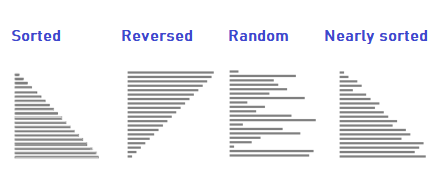
\includegraphics[scale=0.65]{types_of_arrays.PNG}
  % figure captions below figure
  \caption{Different problem types}
  \label{fig:arrays}
\end{figure}

%\begin{figure}
%  \centering
%  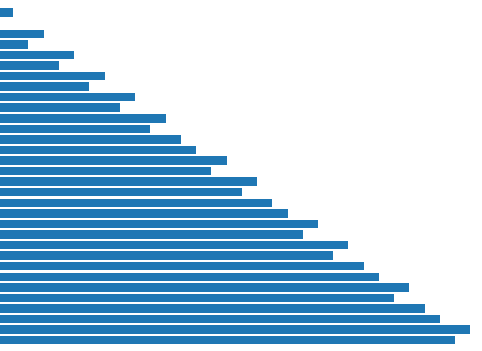
\includegraphics[scale=0.50]{structured array.png}
%  % figure captions below figure
%  \caption{Structured Array}
%  \label{fig:structarr}
%\end{figure}

\subsubsection{Creation of the Arrays}\label{sec:createarrays}

Sorted and Reversed were made using NumPy arrange method. Random and Integers were created using the random number generator of the ArrayGenerator class \cite{RandomGe86:online}. The nearly sorted array or the structured array was generated using sorted inpuut array and a shuffle range used for inplace shuffling of the indices given by equation~\ref{eq:shuffle} and gave an array as shown in figure ~\ref{fig:arrays}.
\begin{equation}
\label{eq:shuffle}
    S = \lfloor 2 *\frac{ 2^n }{n^2}\rfloor, \quad \textit{where} \quad n\textit{ is a power of 2} \land S\textit{ is shuffle range}
\end{equation}

%\begin{listing}[]
%  % Listing captions above the listing.   
%  \caption{Excerpt from ArrayGenerator in utility.py}
%  \label{lst:nearlysorted}
%  \begin{lstlisting}
%ArrayGenerator.structured_array(self, n):
%    A = np.arange(0, int(2**n))
%    # Shuffle range
%    s_r = int(((2**n))//((n**2)/2))
%    for i in range(0, int(2**n), s_r):
%        #In place shuffle within indices
%        self.rng.shuffle(A[i: i + s_r])
%    return A.astype('int32')
%   
%  \end{lstlisting}
%\end{listing}

The Structured Array was shuffled for any array with number of elements $> 0$ since $S$ has it's minimum at $n = 3 \Rightarrow \text{ShuffleRange} = int(1.7778) = 2$

\subsection{Runtime Benchmarking}\label{sec:methbench}

The main bunch of work was done by the $repeating\_timer$ decorator in \texttt{\detokenize{src/utility.py}}, which can be used with single or multiple algorithms (as a callable) several times on the same array. It handled in-place algorithms by assigning a new copy before every iteration, and thereafter saved the results from every iteration in a dictionary with algorithm name as the key and the list of timings as the value. 

%\begin{listing}
%  % Listing captions above the listing.   
%  \caption{Excerpt from repeating\texttt{\detokenize{_}}timer %decorator in %utility.py}
%  \label{lst:timing_dec}
%  \begin{lstlisting}
%    for algo in kwargs [' function_list']:
%    array_copy = copy ( kwargs ['array '])
%    record [ algo . __name__ ] = []
%    for _ in range ( iters ):
%        start_time = time . perf_counter ()
%        algo ( array_copy ) # Exec algorithm
%        end_time = time . perf_counter ()
%        run_time = end_time - start_time
%        record [ algo . __name__ ]. append ( run_time )
%        array_copy = copy ( kwargs ['array '])
%  \end{lstlisting}
%\end{listing}

To generate results \texttt{\detokenize{notebook/generate_data_script.py}} was used. Over time multiple results were generated, and merged together with \texttt{\detokenize{src/merge_csv.py}}, which gave \texttt{\detokenize{data/merged_results.csv}} as an output.
All data points were stored with equality, which then was easy to manipulate when creating new variables and during plotting. See table ~\ref{tab:DF}.

%To keep us updated on how the benchmark was doing while running, we could %look at the terminal outputs shown in figure  ~\ref{fig:outputterminal}.

%\begin{figure}[H]
%    \centering
%    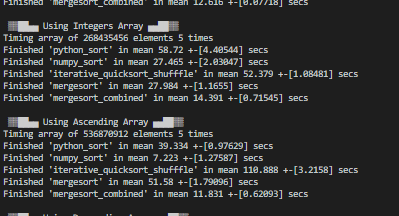
\includegraphics[scale=0.8]{output_to_terminal.PNG}
%    \caption{Terminal output}
%    \label{fig:outputterminal}
%\end{figure}

\subsubsection{Computer and software}\label{sec:comp} OS: Windows 10, Python version 3.7.9, 
Processor:	Intel(R) Core(TM) i5-8250U CPU @ 1.60GHz, 1801 Mhz, 4 cores, 8 logic threads.
8 GB of installed RAM. 
\textbf{Make and model:} Huawei MateBook X Pro i5 dGPU 8GB 256GB (2018)

\subsubsection{GitLab}\label{sec:comp} Git hashes for more details on the code used are provided in table ~\ref{tab:hashes}.

\begin{table}
  % Table captions always come *above* the table.
  \caption{Five random samples from results}
  \label{tab:DF}
\begin{tabular}{ |p{2cm}||p{0.5cm}|p{2cm}|p{2cm}|  }
 \hline
 \multicolumn{4}{|c|}{Results DataFrame} \\
 \hline
 Algorithm & $2^N$ & TypeArray & Time \\
 \hline
 \texttt{\detokenize{python_sort}}&15&Integers& 0.003036\\
 \texttt{\detokenize{numpy_sort}}&21  & Descending & 0.028119\\
  \texttt{\detokenize{numpy_sort}}&1 & Structured& 0.000002\\
 \texttt{\detokenize{numpy_sort}}&15 & Random& 0.002030\\
 \texttt{merge sort}&15& Structured& 0.002981\\
 \hline
\end{tabular}
\end{table}

\begin{table}
  % Table captions always come *above* the table.
  \caption{Versions of files used for this report; {\href{https://gitlab.com/nmbu.no/emner/inf221/h2020/student-term-papers/team_19/inf221-term-paper-team19}{Team 19 gitlab repository}}.}
  \label{tab:hashes}
  \begin{tabular}{ll}
    \hline
    File & Git hash \\\hline
    \verb!src/utility.py! & \verb!04c0a468! \\
    \verb!src/*!        //algorithms and tests & \verb!04c0a468! \\
    \verb!notebooks/generate_data_script.py! & \verb!3f422550! \\
    \verb!notebooks/plot_creation.ipynb! & \verb!520dc68e! \\
    \verb!notebooks/opt_thresh_combined.ipynb! & \verb!8ec07210f! \\
    \verb!data/merged_results.csv! & \verb!88c28d55c! \\
    \verb!asymptotic_bounds/*! & \verb!aa0b819e! \\\hline
  \end{tabular}
\end{table}

\subsection{Challenges and Solutions}\label{sec:challenges&solutions}

\subsubsection{Challenges:}\label{sec:challenges} Various challenges that arouse during the benchmarking process are listed below.

\begin{enumerate}
\item Time taken to benchmark algorithms.
\item Quick sort was problematic with standard implementation. This caused recursion limits and made it difficult to plot against other algorithms. This was mainly due to worst-case partitioning and Python not optimizing tail recursion \cite{Neopytho23:online}. 
\item Finding the threshold for merge sort combined.
\item Verifying the functionality of the sorting algorithms.

\end{enumerate}

\subsubsection{Solutions:}\label{sec:solutions} These implementations were made in order to solve the challenges listed in section ~\ref{sec:challenges}.

\begin{enumerate}
\item JIT-compiled sorting algorithms (effects negatively only on the first calls to the algorithms.) One could have compiled ahead of time, but since that caused complication with data types and what OS or Hardware one is running, we JIT-compiled every algorithm except NumPy sort.
\item Iterative quick sort was implemented with median of three partitioning. This led to only iterative quick sort with median of three pivot optimization being used instead, for all benchmarking. There are other ways to handle the recursion depth issue, but they would stray far away from the standard quick sort. For example hybrid with heap or binary insertion sort, or multi-pivot partitioning.
\item The largest $\frac{\delta(a, b)}{\delta(n)}$ where a is time taken by merge sort and b is insertion sort, was found. Which in this case was a threshold of 142. Hence, each split of merge sort with n < threshold was sorted using insertion sort. See figure ~\ref{fig:ins_merge_opt} and section ~\ref{sec:res_optimize}. Another way to find the threshold dynamically could be with something similar to timsort's minrun size as described shortly in section ~\ref{sec:algo6}.  

\item Unittests in tests/test\_algos.py

\end{enumerate}

\section{Results}\label{sec:results}
The following section is dedicated to presenting visual results of the algorithms listed in section~\ref{sec:intro}. The y-axis of all plots in the results section is runtime divided by N-length of arrays measured in microseconds, except for figure ~\ref{fig:ins_merge_opt} which is time measured in seconds. 

\subsection{Optimal Threshold for Merge Sort Combined}\label{sec:res_optimize}

This result is a dependency of the selected threshold in merge sort combined. If more details surrounding this is of interest, look up: \texttt{\detokenize{notebook/opt_thresh_combined.ipynb}}, to see how the results were generated. 

Figure ~\ref{fig:ins_merge} are increments of 1 from 25 to 200 showing the different types of input arrays for merge and insertion sort. The colored bands show the standard deviation for each algorithm.

Figure ~\ref{fig:ins_merge_opt} shows the mean aggregated over algorithm and N, giving a single line representing the average-case. It also shows the threshold value for insertion sort. Below the array length of 300 elements, insertion sorts performs better than merge sort.

\begin{figure}[H]
  \centering
  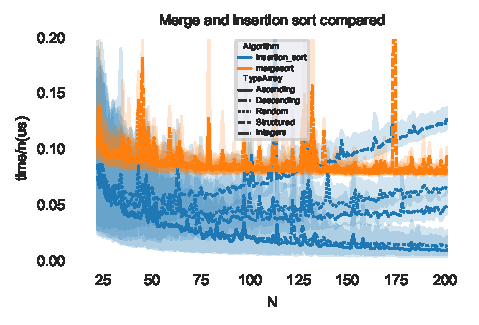
\includegraphics[scale=0.95]{optimizing.pdf}
  % figure captions below figure
  \caption{Comparing insertion sort with merge sort}
  \label{fig:ins_merge}
\end{figure}

\begin{figure}[]
  \centering
  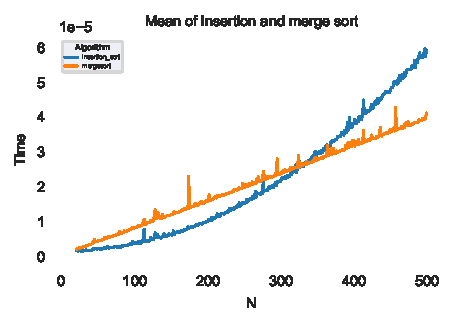
\includegraphics[scale=0.75]{optimizing_combined_threshold.pdf}
  % figure captions below figure
  \caption{Comparing insertion sort with merge sort}
  \label{fig:ins_merge_opt}
\end{figure}

\subsection{Benchmarking Individual Algorithms}\label{sec:results_ind}
The results of the individual algorithms with different array sizes and types are presented in figures ~\ref{fig:time_per_nbubble_sort}, ~\ref{fig:time_per_ninsertion_sort},
~\ref{fig:time_per_npython_sort}, ~\ref{fig:time_per_niterative_quicksort},  ~\ref{fig:time_per_nmergesort}, ~\ref{fig:time_per_nmergesort_combined} and ~\ref{fig:time_per_nnumpy_sort}. 

Insertion sort~\ref{fig:time_per_ninsertion_sort} and bubble sort~\ref{fig:time_per_nbubble_sort}, displayed quadratic growth, and interestingly bubble sort performed around 100 seconds faster than insertion sort on descending arrays, when $N=2^{20}$. Insertion sort performs well on ascending and structured data.


\begin{figure}[]
  \centering
  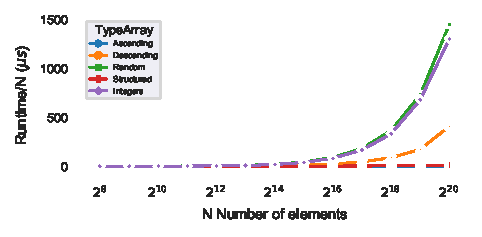
\includegraphics[scale=0.75]{time_per_nbubble_sort.pdf}
  % figure captions below figure
  \caption{Bubble Sort}
  \label{fig:time_per_nbubble_sort}
\end{figure}

\begin{figure}[]
  \centering
  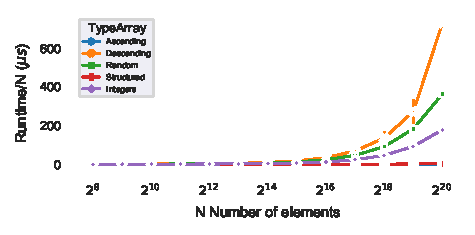
\includegraphics[scale=0.75]{time_per_ninsertion_sort.pdf}
  % figure captions below figure
  \caption{Insertion Sort}
  \label{fig:time_per_ninsertion_sort}
\end{figure}


\begin{figure}[]
  \centering
  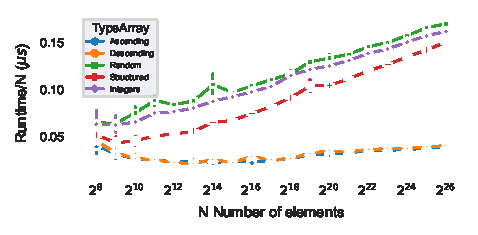
\includegraphics[scale=0.75]{time_per_npython_sort.pdf}
  % figure captions below figure
  \caption{Python Sort}
  \label{fig:time_per_npython_sort}
\end{figure}

Python sort~\ref{fig:time_per_npython_sort} performed in sub-quadratic time on structured and randomized input arrays. One can observe linear growth on ascending and descending input arrays, which with the selected y-axis is approximately a horizontal line.

Iterative quick sort, shown in figure~\ref{fig:time_per_niterative_quicksort}, produced similar behaviour to python sort, but descending arrays give sub-quadratic time complexity and the ascending input arrays looks almost linear. Keep in mind that this implementation is with median of three pivot.

\begin{figure}[]
  \centering
  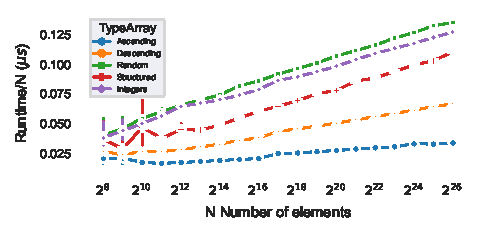
\includegraphics[scale=0.75]{time_per_niterative_quicksort.pdf}
  % figure captions below figure
  \caption{Iterative Quick Sort}
  \label{fig:time_per_niterative_quicksort}
\end{figure}

\begin{figure}[]
  \centering
  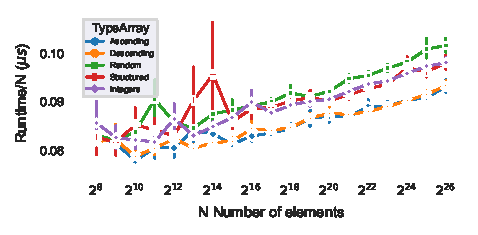
\includegraphics[scale=0.75]{time_per_nmergesort.pdf}
  % figure captions below figure
  \caption{Merge Sort}
  \label{fig:time_per_nmergesort}
\end{figure}

In figure ~\ref{fig:time_per_nmergesort} one can see broad error bars for merge sort before it balances out after $2^{14}$ elements. Every array type induces $n\lg(n)$ growth with varying constants as with Python sort and iterative quick sort. 

\begin{figure}[]
  \centering
  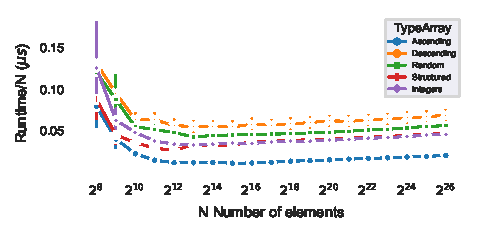
\includegraphics[scale=0.75]{time_per_nmergesort_combined.pdf}
  % figure captions below figure
  \caption{Merge Sort Combined}
  \label{fig:time_per_nmergesort_combined}
\end{figure}

Merge sort combined looks deceivingly like it has linear growth, this is not the case. One can observe very small constants in figure ~\ref{fig:time_per_nmergesort_combined}. It uses between 2 to 10 as much time per elements with arrays of size $2^8$, compared to arrays larger than $2^{14}= 16,384$.

NumPy sort's results, shown in figure~\ref{fig:time_per_nnumpy_sort}, looks quite similar to python sort just with a lower y-axis. 

\begin{figure}[H]
  \centering
  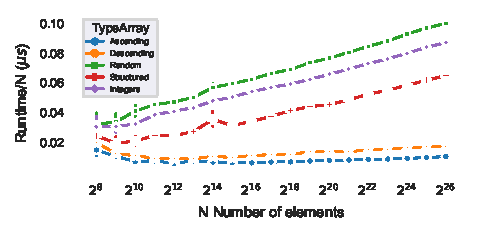
\includegraphics[scale=0.75]{time_per_nnumpy_sort.pdf}
  % figure captions below figure
  \caption{NumPy Sort}
  \label{fig:time_per_nnumpy_sort}
\end{figure}

\subsection{Comparing Algorithms}\label{sec:results_comp}

The first two algorithms compared were the quadratic sorting algorithms shown in figure~\ref{fig:bubble_insertion}. Insertion sort clearly performs better for all types of arrays except for ascending arrays, and descending described in section ~\ref{sec:results_ind} . It is possible to zoom in on the PDF to see the plot distinctions better. 

Figure~\ref{fig:ins_merge} shows a comparison of merge sort and insertion sort, as mentioned in section~\ref{sec:res_optimize}. Seeing this it is evident that insertion sort is superior in sorting efficiently, compared to merge sort, given the array size. Merge sort however is more consistent in its performance across the different input arrays. 


The next comparison plot, seen in figure~\ref{fig:merge_quick}, is of the sub-quadratic sorting algorithms. Quick sort performs better than merge sort when sorting all arrays up to a length of $2^{15}$. For ascending and descending arrays quick sorts performs the best across all array sizes. However, quick sorts performance also varies a lot depending on the type of the input array. Merge sort on the other hand, stays surprisingly consistent in performance when both the type and size of the input array varies. When the array size approaches a length of $2^{28}$ elements and greater, both the algorithms seemed to struggle. The error bars that occur on the lines early on the x-axis may have been disturbances that occurred while running the benchmarking. 

Comparing merge sort with merge sort combined, seen in figure~\ref{fig:merge_mergecomb}, one can observe that both algorithms have a similar decrease in performance as the array size increases along the x-axis. However, merge sort combined clearly performs better than ordinary merge sort when it comes to all the array types. Another difference is that merge sort combined's performance is less consistent across the types of arrays. It sorts ascending arrays the best. Ordinary merge sort on the other hand performs quite similarly time wise on all the different input arrays. In this plot as well there seems to be a struggle when the array size exceeds a length of $2^{28}$. 

Finally the four best performers are compared; merge sort combined and iterative quick sort are compared to NumPy's and Python's in-place sorts, shown in figure ~\ref{fig:msc_np}, ~\ref{fig:iqs_ps} and ~\ref{fig:mean_np_py_mergecomb}. Figure~\ref{fig:mean_np_py_mergecomb} shows an average-case representation of figures ~\ref{fig:iqs_ps}, ~\ref{fig:msc_np}. In these plots one can see that merge sort combined still is the most consistent both across different types of arrays and also as array size increases. In addition it beats the other algorithms in random, structured and integer arrays. However, NumPy sort is superior when it comes to ascending and descending arrays. In figure~\ref{fig:mean_np_py_mergecomb} we clearly see that NumPy sort and merge sort combined all round are the two best performers, beating both iterative quick sort and Python sort. Python sort is slightly more consistent than iterative quick sort (figure~\ref{fig:iqs_ps}). However, on average iterative quick sort clearly is the better performer of the two (figure~\ref{fig:mean_np_py_mergecomb}).


%\begin{figure*}[]
%\centering
%\subfloat[Subfigure 1 list of figures text][Subfigure 1 %caption]{
%\includegraphics[width=0.38\textwidth]{runtimebubble&ins%ertion.pdf}
%\label{fig:subfig1}}
%\qquad
%\subfloat[Subfigure 2 list of figures text][Subfigure 2 %caption]{
%\includegraphics[width=0.38\textwidth]{runtime_per_n_mer%ge&quick.pdf}
%\label{fig:subfig2}}
%\subfloat[Subfigure 3 list of figures text][Subfigure 3 %caption]{
%\includegraphics[width=0.38\textwidth]{runtime_per_n_mer%ge&combined.pdf}
%\label{fig:subfig3}}
%\qquad
%\subfloat[Subfigure 4 list of figures text][Subfigure 4 %caption]{
%\includegraphics[width=0.38\textwidth]{INF221/runtime_pe%r_n_combined&np.pdf}
%\label{fig:subfig4}}
%\caption{This is a figure containing several %subfigures.}
%\label{fig:globfig}
%\end{figure*}

\begin{figure}[]
  \centering
  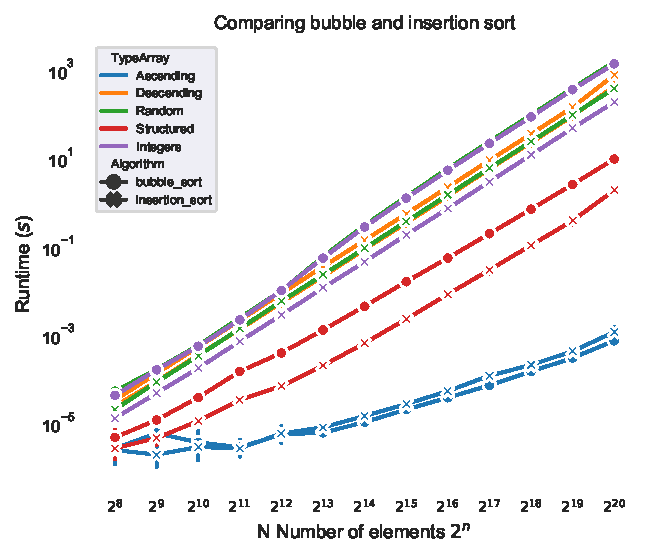
\includegraphics[scale=0.9]{runtimebubble&insertion.pdf}
  % figure captions below figure
  \caption{Insertion sort and bubble sort.}
  \label{fig:bubble_insertion}
\end{figure}

\begin{figure}[]
  \centering
  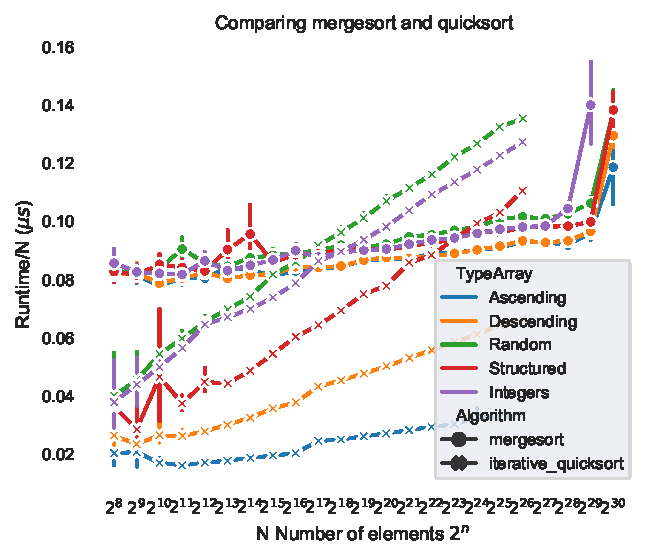
\includegraphics[scale=0.9]{runtime_per_n_merge&quick.pdf}
  % figure captions below figure
  \caption{Merge sort and iterative quick sort.}
  \label{fig:merge_quick}
\end{figure}

\begin{figure}[]
  \centering
  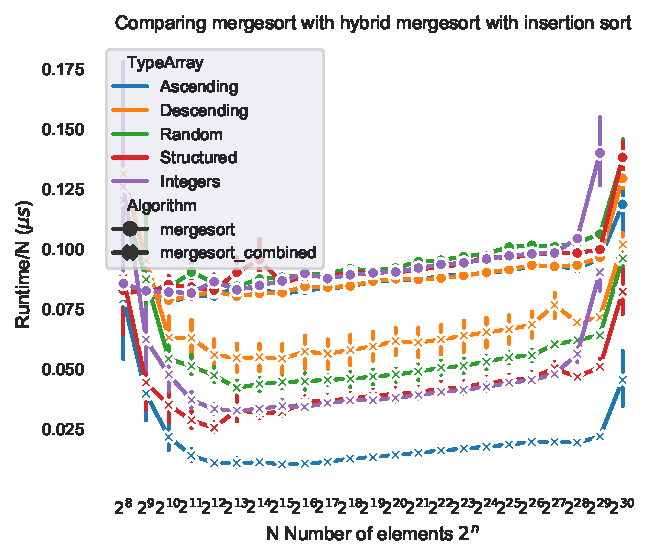
\includegraphics[scale=0.9]{runtime_per_n_merge&combined.pdf}
  % figure captions below figure
  \caption{Merge sort and merge sort combined.}
  \label{fig:merge_mergecomb}
\end{figure}

\begin{figure}[]
  \centering
  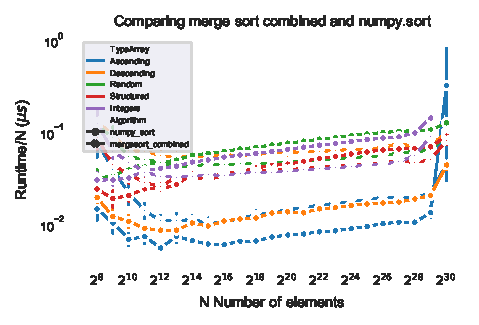
\includegraphics[scale=0.9]{INF221/runtime_per_n_combined&np.pdf}
  % figure captions below figure
  \caption{Merge sort combined and NumPy sort}
  \label{fig:msc_np}
\end{figure}

\begin{figure}[]
  \centering
  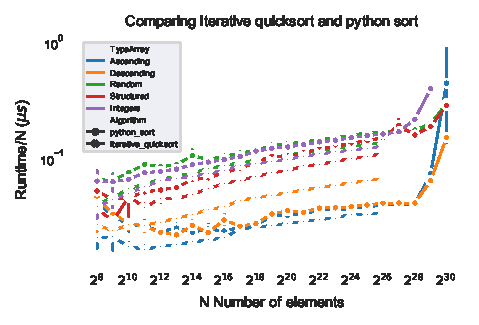
\includegraphics[scale=0.9]{INF221/runtime_per_n_iterqs&py.pdf}
  % figure captions below figure
  \caption{Iterative quick sort and python sort}
  \label{fig:iqs_ps}
\end{figure}

\begin{figure}[]
  \centering
  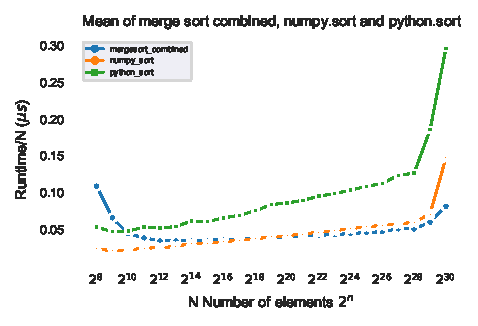
\includegraphics[scale=0.9]{INF221/mean_runtime_per_n_combined&np&py.pdf}
  % figure captions below figure
  \caption{Mean of figures ~\ref{fig:iqs_ps} and ~\ref{fig:msc_np}}
  \label{fig:mean_np_py_mergecomb}
\end{figure}

\subsection{Asymptotic Bounds and Numerical Results}\label{sec:results_comp}
After analysis, table ~\ref{tab:asympt} are the asymptotic bounds for this paper's choice of algorithms. $f(n)$ with $c_1$ is lower bound, and $g(n)$ with $c_2$ is upper bound. 

Presenting table ~\ref{tab:asympt} with $n_0 = 256$. Plots of results can be found in directory \texttt{\detokenize{asymptotic_bounds/*}} in our gitlab repository in table ~\ref{tab:hashes}.

 Denoted with the algorithm's abbreviations, table ~\ref{tab:res_time} displays the average runtime over all different array types and experiments conducted for this paper with the \texttt{\detokenize{notebooks/generate_data_script.py}}. 
 
\begin{table}[]
\centering
\caption{Asymptotic boundaries}
\label{tab:asympt}
\resizebox{\columnwidth}{!}{%

\begin{tabular}{| L | L | L | L | L |}
\textbf{Algorithm} & \textit{f(n)}   & \textit{g(n)}        & c_1         & c_2         \\ \hline
\textit{Bubble sort}        & \Omega(n)       & \mathcal{O}(n^2)     & 3.98 \cdot 10^{-10} & 1.58 \cdot 10^{-9}  \\
\textit{Insertion sort}     & \Omega(n)       & \mathcal{O}(n^2)     & 5.01 \cdot 10^{-10} & 7.94 \cdot 10^{-10} \\
\textit{Iterative QS}        & \Omega(n\lg(n)) & \mathcal{O}(n\lg(n))     & 1.00 \cdot 10^{-9}  & 5.01 \cdot 10^{-9}  \\
\textit{Merge sort}         & \Omega(n\lg(n)) & \mathcal{O}(n\lg(n)) & 2.51 \cdot 10^{-9}  & 6.31 \cdot 10^{-9}  \\
\textit{MS combined}        & \Omega(n\lg(n)) & \mathcal{O}(n\lg(n)) & 5.01 \cdot 10^{-10} & 3.16 \cdot 10^{-10} \\
\textit{NumPy sort}         & \Omega(n\lg(n))       & \mathcal{O}(n\lg(n)) & 3.98 \cdot 10^{-10}  & 6.31 \cdot 10^{-9}  \\
\textit{Python sort}        & \Omega(n)       & \mathcal{O}(n\lg(n)) & 2.00 \cdot 10^{-8}  & 1.00 \cdot 10^{-8} 
\end{tabular}
}
\end{table}

\begin{table}
\centering
\caption{Average runtimes of algorithms (Time in (S))}
\label{tab:res_time}
\resizebox{\columnwidth}{!}{%
\begin{tabular}{lrrrrrrr}

\toprule
\textbf{Algorithm} &  BS &  IS &  IQS &  MS &  MSC &  NS &  PS \\
\textbf{$2^N$} &              &                 &                      &            &                     &             &              \\
\midrule
2   &      0.00000 &         0.00000 &              0.00000 &    0.00000 &             0.00002 &     0.00000 &      0.00000 \\
4   &      0.00000 &         0.00000 &              0.00000 &    0.00000 &             0.00002 &     0.00000 &      0.00001 \\
6   &      0.00000 &         0.00000 &              0.00000 &    0.00001 &             0.00002 &     0.00000 &      0.00001 \\
8   &      0.00003 &         0.00001 &              0.00001 &    0.00002 &             0.00003 &     0.00001 &      0.00001 \\
10  &      0.00031 &         0.00021 &              0.00004 &    0.00008 &             0.00005 &     0.00002 &      0.00005 \\
12  &      0.00521 &         0.00350 &              0.00018 &    0.00034 &             0.00014 &     0.00010 &      0.00021 \\
14  &      0.13483 &         0.05552 &              0.00080 &    0.00142 &             0.00058 &     0.00051 &      0.00101 \\
16  &      2.52257 &         0.88911 &              0.00372 &    0.00570 &             0.00241 &     0.00219 &      0.00432 \\
18  &     41.11392 &        14.26344 &              0.01709 &    0.02310 &             0.01005 &     0.00985 &      0.01979 \\
20  &    666.04966 &       267.50417 &              0.07563 &    0.09390 &             0.04230 &     0.04384 &      0.09039 \\
22  &          nan &             nan &              0.33473 &    0.38491 &             0.17768 &     0.19543 &      0.40016 \\
24  &          nan &             nan &              1.46942 &    1.58280 &             0.75032 &     0.86001 &      1.73815 \\
26  &          nan &             nan &              6.35141 &    6.49816 &             3.17001 &     3.74989 &      7.55585 \\
28  &          nan &             nan &                  nan &   26.35145 &            13.65878 &    16.14606 &     34.00469 \\
30  &          nan &             nan &                  nan &  140.68718 &            87.54823 &   158.28938 &    317.99038 \\
\bottomrule
\end{tabular}
}
\end{table}



\section{Discussion}\label{sec:discussion}

As mentioned, the quadratic sorting algorithms are the slowest algorithms, which is as expected considering they both have the slowest average runtime of $\Theta(n^2)$. Which is confirmed when seeing their quadratic curves in the individual benchmark-plots (figure~\ref{fig:time_per_nbubble_sort} and ~\ref{fig:time_per_ninsertion_sort}). 

Even though there are many more powerful algorithms than insertion sort, such as merge sort, the time cost caused by the large overhead results in them failing to beat insertion sort when sorting smaller arrays. In this case the threshold being around 300 elements. This is supported by the results in figure~\ref{fig:ins_merge}, which coincides with the theory from section~\ref{sec:algo3}. Bringing us to the reason why insertion sort is often used internally in other sorting algorithms, as it is highly efficient in sorting small portions of the input array, ultimately resulting in even better performing hybrid algorithms. Such as timsort or merge sort combined for instance.

In figure ~\ref{fig:merge_quick} we saw that quick sort performs the best on ascending and descending arrays. In theory section~\ref{sec:algo4} we mentioned that these arrays were two of the worst case scenarios for quick sort with last pivot partitioning. The fact that quick sort performs this well when these arrays means that the pivot optimization and the iterative implementation of quick sort is successful in handling the recursion issues that normally would arise when sorting such problems. In fact, quick sort even outperforms Python sort for all input arrays except descending, as seen in figure~\ref{fig:iqs_ps}. The reason Python sort performs better for descending arrays is probably due to the ability of the minruns to detect smaller portions of the input array being in reverse order. Resulting in Python sort reversing the array in linear time. 

Figure ~\ref{fig:merge_quick} and table~\ref{tab:asympt} also shows that there are obvious performance differences between algorithms even though they are within the same complexity class, which is $\Theta(n\lg n)$ in this case.

As mentioned in the results, many of the algorithms 'struggled' towards the end of the plots. They increased in runtime by a factor between 2 and 10 as the array size reached a length of $2^{29}$ to $2^{30}$ on the x-axis. This is because the RAM of the simulation computer was filled, and the memory was then shifted between physical memory and virtual memory. This means we should take the results after $2^{28}$ with a grain of salt, since other factors as which order they are benchmarked might affect the results. It can also be favoring algorithms with non linear space complexity and/or small overhead. 

Overall, the experimental results coincide well with the theoretical runtime assumptions. Although the self implemented algorithms perform much better than expected. Two out of the four best performing algorithms were as expected the built-in NumPy and Python sort (figure~\ref{fig:mean_np_py_mergecomb}). However, Python sort only performs the fourth best until a certain array length, after which it is beaten by ordinary merge sort. When the input array length exceeds $2^{20}$, ordinary merge sort becomes the fourth best performing algorithm, as seen in table ~\ref{tab:res_time}. The fact that the implementations of both merge sort and merge sort combined performed nearly as well as NumPy sort, and in fact even beats NumPy sort at the end of the benchmarking (table~\ref{tab:res_time}), is quite shocking. Although, one should be slightly apprehensive towards the benchmarking results passing an array length of $2^{28}$. 

This of course makes one wonder how the self-implemented algorithms perform so well in comparison to the NumPy and Python built-in-sort's. Using Numba, the slowdown of the algorithms implemented in pure Python code versus the built-in ones, is nearly eliminated. Which most probably is a large reason to why these results were obtained.

Finally, the two best performers; NumPy sort and merge sort combined, all have in common that they are hybrid algorithms. This goes to show that combining efficient sorting algorithms, and when implemented with suitable thresholds and compilation, results in superior performance.

Due to time and space constrictions we did not test the algorithms on arrays with many duplicate elements nor string. However, this could potentially be interesting to investigate in further explorations. Testing hybridization's of different algorithms with a greater number of array types, and specific worst-case ``killer-problems'', for the different algorithms, would be a worthwhile investigation.

% In the acks section, you can thank people for help.
\begin{acks}

We are grateful to Khariton Gorbunov and Mathias Chunnoo for guidance. Bao Ngoc Huynh for good feedback on drafts. Fabian Nemazi for useful discussion and advice. Last but not least, we are thankful for the knowledge, interesting lectures and guidance provided by Hans Ekkehard Plesser.

\end{acks}

%% The next two lines define the bibliography style to be used, and
\bibliographystyle{ACM-Reference-Format}
\bibliography{term_paper_bib}

\end{document}
